\documentclass[t]{beamer}

% Load general definitions
% Preamble file - general definitions, package loading, etc.

%=================================
% Load packages
\usepackage{amssymb,amsmath}
\usepackage{graphicx}
\usepackage{url}
\usepackage{tikz}
\usetikzlibrary{mindmap,trees,arrows}
\usepackage{fancyvrb}
\usepackage[portuguese]{babel} 
\usepackage[utf8]{inputenc}
\usepackage{subfigure}
\usepackage{times}
\usepackage[T1]{fontenc}
\usepackage{cancel}
\usepackage{color}
\usepackage{listings}
\usepackage[document]{ragged2e}

%=================================
% Set mode
\mode<presentation>
{
	\usetheme{Madrid}
	\usecolortheme{structure}
	\useoutertheme{infolines}
	\setbeamercovered{invisible}
}

% Get rid of nav bar
\beamertemplatenavigationsymbolsempty

% Insert frame number at bottom of the page.
\usefoottemplate{\hfil\tiny{\color{black!90}\insertframenumber}} 

%=================================
% Define new commands

\newcommand\Real{{\mathbb{R}}}
%\newcommand{\vi}{\vspace{0.6\baselineskip}}
%\newcommand{\goodgap}{\hspace{\subfigtopskip}\hspace{\subfigbottomskip}}


% Equation environments
\newcommand{\beq}{\begin{equation}}
\newcommand{\eq}{\end{equation}}
\newcommand{\beqs}{\begin{equation*}}
\newcommand{\eqs}{\end{equation*}}
\newcommand{\beqn}{\begin{eqnarray}}
\newcommand{\eqn}{\end{eqnarray}}
% Bold variables
\newcommand{\mbf}[1]{\ensuremath{\mathbf{#1}}}
% Itemization
\newcommand{\bitem}{\begin{itemize}}
\newcommand{\eitem}{\end{itemize}}
\newcommand{\spitem}{\vskip 1em\item}
\newcommand{\bitems}{\begin{itemize}\item}
\newcommand{\benums}{\begin{enumerate}\item}
\newcommand{\eenum}{\end{enumerate}}
% color blocks
\newenvironment{colorblock}[2]{%
\setbeamercolor{block title}{#2}
\begin{block}{#1}}{\end{block}}
% Vertical spacing
\newcommand{\vone}{\vskip 1em}
\newcommand{\vhalf}{\vskip .5em}
% Frame environments
\newenvironment{ftst}[3][t]{%
\begin{frame}{environment=ftst,#1}
\frametitle{#2}
\framesubtitle{#3}}{\end{frame}}
\newenvironment{ftstf}[2]{
\begin{frame}[fragile,environment=ftstf]
\frametitle{#1}
\framesubtitle{#2}}{\end{frame}}
% colors
\definecolor{MyGray}{rgb}{0.5,0.5,0.5}
\definecolor{MyDBGray}{rgb}{0.1,0.1,0.4}
\definecolor{darkgreen}{rgb}{0,0.4,0}
\definecolor{black}{rgb}{0,0,0}
\def\defn#1{{\color{red} #1}}
% Footnote
\renewcommand{\thefootnote}{\alph{footnote}}
% Relaxed footnotes
\newcommand{\lfr}[1]{\let\thefootnote\relax\footnote{\tiny #1}}
% Verbatim environment - using FANCYVRB package
\DefineVerbatimEnvironment%
{rcode}{Verbatim}
{fontsize=\scriptsize}
% Verbatim environment - using LISTINGS package
%\lstnewenvironment{rcode} {\lstset{	language = R,
%									basicstyle = \scriptsize\ttfamily,
%									showspaces = false,
%									showstringspaces = false,
%									showtabs = false,
%									keywordstyle = \color{black}\bfseries,
%									commentstyle = \color{darkgreen},
%									numbers = none,
%									otherkeywords={	<-,
%													ggplot,
%													geom_boxplot,
%													facet_grid,
%													shapiro.test,
%													fligner.test,
%													glht,
%													with},
%									deletekeywords={data,
%													model,
%													residuals,
%													c,
%													axis,
%													default,
%													labels,
%													qq.text}}}%
%{}

% Specific definitions
\title[]{Algoritmos e Estruturas de Dados III}
\subtitle[]{Introdução à Teoria dos Grafos}
\author[]{Patrícia Lucas\\{\footnotesize }}
\institute{Bacharelado em Sistemas de Informação \\ IFNMG  - Campus Salinas}
\date{\scriptsize Salinas\\Dezembro 2020}

\begin{document}

% cover page
\setbeamertemplate{footline}{}
\begin{frame}

\begin{center}
\includegraphics[width=.15\textwidth]{}
\end{center}
  \titlepage
  \begin{tikzpicture}[remember picture,overlay]
  \node[anchor=south east,xshift=-5pt,yshift=5pt] at (current page.south east) {\tiny Versão 1.2020};
  \node[anchor=south west,yshift=0pt] at (current page.south west) {
\includegraphics[width=.25\textwidth]{Logos/salinas_horizontal_jpg.jpg}};
  \end{tikzpicture}  
\end{frame}

% Main slides
\begin{ftst}{Conceito}{Teoria dos grafos}

\begin{itemize}
    \item A teoria dos grafos é um subconjunto da matemática discreta. 
    \item Um grafo é usado para modelar coisas que têm relações com outras coisas - essa definição vaga sugere a enorme flexibilidade dos grafos na resolução de problemas. 
    \item O notável poder da teoria dos grafos foi usado para resolver problemas em praticamente todas as áreas.
\end{itemize}

\end{ftst}

%=====

\begin{ftst}{Terminologia}{Teoria dos grafos}

Um grafo simples $G =(V,E)$ consiste de um conjunto não vazio $V$ de vértices e um conjunto que pode ou não ser vazio $E$ de arestas, cada aresta sendo um conjunto de dois vértices $(v_i, v_j)$ a partir de $V$, sendo $(v_i,v_j)=(v_j,v_i)$. \\
\vone
O número de vértices e arestas é denotado por $|V|$ e $|E|$, respectivamente.

\centering 

\tikzset{every picture/.style={line width=0.75pt}} %set default line width to 0.75pt        

\begin{tikzpicture}[x=0.75pt,y=0.75pt,yscale=-1,xscale=1]
%uncomment if require: \path (0,125); %set diagram left start at 0, and has height of 125

%Shape: Ellipse [id:dp56526211521717] 
\draw  [fill={rgb, 255:red, 0; green, 0; blue, 0 }  ,fill opacity=1 ] (46.35,48.98) .. controls (46.35,44.17) and (50.56,40.28) .. (55.75,40.28) .. controls (60.94,40.28) and (65.15,44.17) .. (65.15,48.98) .. controls (65.15,53.79) and (60.94,57.69) .. (55.75,57.69) .. controls (50.56,57.69) and (46.35,53.79) .. (46.35,48.98) -- cycle ;
%Shape: Ellipse [id:dp704999339935936] 
\draw  [fill={rgb, 255:red, 0; green, 0; blue, 0 }  ,fill opacity=1 ] (100.36,99.41) .. controls (100.36,94.6) and (104.57,90.71) .. (109.76,90.71) .. controls (114.95,90.71) and (119.15,94.6) .. (119.15,99.41) .. controls (119.15,104.22) and (114.95,108.11) .. (109.76,108.11) .. controls (104.57,108.11) and (100.36,104.22) .. (100.36,99.41) -- cycle ;
%Shape: Ellipse [id:dp18766605151664573] 
\draw  [fill={rgb, 255:red, 0; green, 0; blue, 0 }  ,fill opacity=1 ] (105.31,49.67) .. controls (105.31,44.86) and (109.52,40.97) .. (114.71,40.97) .. controls (119.9,40.97) and (124.11,44.86) .. (124.11,49.67) .. controls (124.11,54.48) and (119.9,58.37) .. (114.71,58.37) .. controls (109.52,58.37) and (105.31,54.48) .. (105.31,49.67) -- cycle ;
%Shape: Ellipse [id:dp860106873164983] 
\draw  [fill={rgb, 255:red, 0; green, 0; blue, 0 }  ,fill opacity=1 ] (74.61,67.65) .. controls (74.61,62.84) and (78.82,58.94) .. (84.01,58.94) .. controls (89.2,58.94) and (93.4,62.84) .. (93.4,67.65) .. controls (93.4,72.45) and (89.2,76.35) .. (84.01,76.35) .. controls (78.82,76.35) and (74.61,72.45) .. (74.61,67.65) -- cycle ;
%Shape: Ellipse [id:dp9624212908786325] 
\draw  [fill={rgb, 255:red, 0; green, 0; blue, 0 }  ,fill opacity=1 ] (22.17,75.88) .. controls (22.17,71.07) and (26.38,67.17) .. (31.57,67.17) .. controls (36.76,67.17) and (40.96,71.07) .. (40.96,75.88) .. controls (40.96,80.68) and (36.76,84.58) .. (31.57,84.58) .. controls (26.38,84.58) and (22.17,80.68) .. (22.17,75.88) -- cycle ;
%Shape: Ellipse [id:dp666723248449479] 
\draw  [fill={rgb, 255:red, 0; green, 0; blue, 0 }  ,fill opacity=1 ] (76.05,15.56) .. controls (76.05,10.75) and (80.26,6.85) .. (85.45,6.85) .. controls (90.64,6.85) and (94.85,10.75) .. (94.85,15.56) .. controls (94.85,20.37) and (90.64,24.26) .. (85.45,24.26) .. controls (80.26,24.26) and (76.05,20.37) .. (76.05,15.56) -- cycle ;
%Shape: Ellipse [id:dp9741887195317744] 
\draw  [fill={rgb, 255:red, 0; green, 0; blue, 0 }  ,fill opacity=1 ] (29.06,13.82) .. controls (29.06,9.01) and (33.27,5.11) .. (38.46,5.11) .. controls (43.65,5.11) and (47.86,9.01) .. (47.86,13.82) .. controls (47.86,18.62) and (43.65,22.52) .. (38.46,22.52) .. controls (33.27,22.52) and (29.06,18.62) .. (29.06,13.82) -- cycle ;
%Shape: Ellipse [id:dp5101164697169429] 
\draw  [fill={rgb, 255:red, 0; green, 0; blue, 0 }  ,fill opacity=1 ] (5,40.28) .. controls (5,35.47) and (9.21,31.57) .. (14.4,31.57) .. controls (19.59,31.57) and (23.8,35.47) .. (23.8,40.28) .. controls (23.8,45.08) and (19.59,48.98) .. (14.4,48.98) .. controls (9.21,48.98) and (5,45.08) .. (5,40.28) -- cycle ;
%Straight Lines [id:da6271899558210341] 
\draw [fill={rgb, 255:red, 0; green, 0; blue, 0 }  ,fill opacity=1 ]   (29.55,71) -- (17.14,46.21) ;
%Straight Lines [id:da2230066147300016] 
\draw [fill={rgb, 255:red, 0; green, 0; blue, 0 }  ,fill opacity=1 ]   (19.9,32.51) -- (30.92,20.12) ;
%Straight Lines [id:da5606460186184359] 
\draw    (47.47,10.33) -- (76.42,11.64) ;
%Straight Lines [id:da6611820119232676] 
\draw    (38.51,69.7) -- (51.6,55.35) ;
%Straight Lines [id:da8708544360856261] 
\draw    (61.25,42.3) -- (79.86,22.08) ;
%Straight Lines [id:da4619727420957742] 
\draw    (89.51,20.12) -- (111.57,45.56) ;
%Straight Lines [id:da7644501958337031] 
\draw    (85.45,15.56) -- (84.01,67.65) ;
%Straight Lines [id:da22348802745324092] 
\draw    (31.57,75.88) -- (109.76,99.41) ;
%Straight Lines [id:da6696267389895008] 
\draw    (84.01,67.65) -- (109.76,99.41) ;
%Straight Lines [id:da6177319913365642] 
\draw    (114.71,49.67) -- (109.76,99.41) ;




\end{tikzpicture}
Exemplo: Grafo com $|V| = 8$ e $|E| = 10$

\end{ftst}

%=====

\begin{ftst}{Aplicações}{Teoria dos grafos}
\justifying
\begin{itemize}
    \item O projeto do sistema de água municipal utiliza a teoria dos grafos para modelar o fluxo de água para garantir que os requisitos de pressão sejam atendidos.
    \item Redes sociais como Facebook e Twitter usam a teoria dos grafos para sugerir amigos e vender anúncios.
    \item A Netflix usa a teoria dos grafos para recomendar filmes.
    \item O Google Maps usa a teoria dos grafos para encontrar o caminho mais curto da sua casa até o seu destino.
    \item A infraestrutura da Internet se baseia na teoria dos grafos para rotear seu tráfego de nó em nó na infraestrutura física da internet.
    \item Os engenheiros de videogame usam a teoria dos grafos para direcionar os NPCs (personagens não jogadores) por seus mundos virtuais.
\end{itemize}

\end{ftst}

%=====

\begin{ftst}{Aplicações}{Teoria dos grafos}
\vone
\vone
\centering
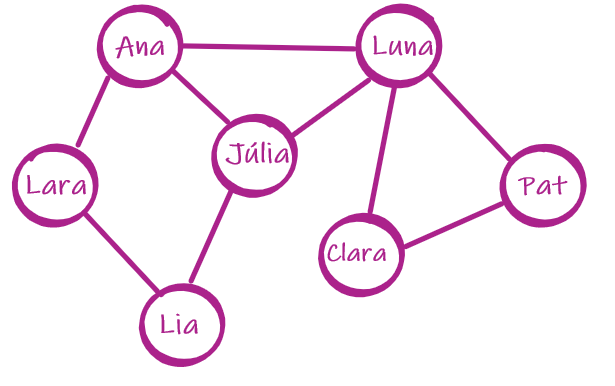
\includegraphics[scale=0.5]{Figuras/redes.png}\\
\vone
\vone
Representação da relação entre pessoas numa rede social.

\end{ftst}

%=====

\begin{ftst}{Aplicações}{Teoria dos grafos}
\vone
\vone
\centering
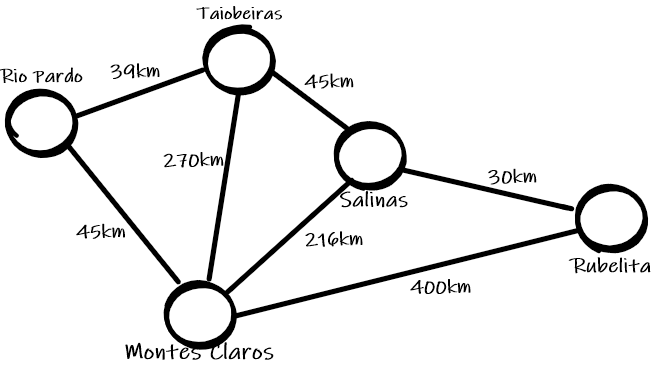
\includegraphics[scale=0.5]{Figuras/cidades.png}\\
\vone
\vone
Representação da ligação entre cidades e suas distâncias.
\end{ftst}

%=====

\begin{ftst}{Dígrafos}{Teoria dos grafos}
\justifying
Um \textbf{dígrafo} ou \textbf{grafo dirigido} consiste de um conjunto não vazio $V$ de vértices e um conjunto $E$ de arestas (que também podem ser chamadas de arcos), onde cada aresta é da forma $(v_i,v_j)$, sendo: $(v_i,v_j) \neq (v_j,v_i)$.
\vone

\centering
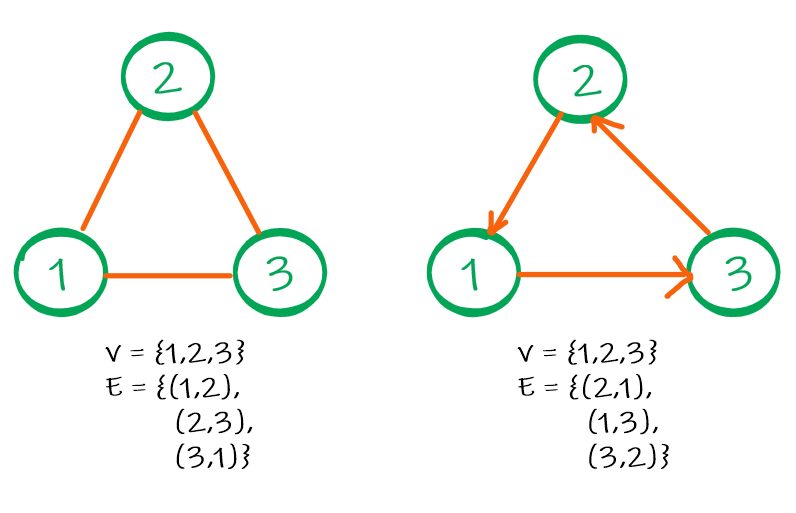
\includegraphics[scale=0.5]{Figuras/graph_digrafo.png}\\

\end{ftst}

%=====

\begin{ftst}{Dígrafos}{Teoria dos grafos}
\centering
\textbf{Facebook x Twitter}

\vone

\vone
\centering
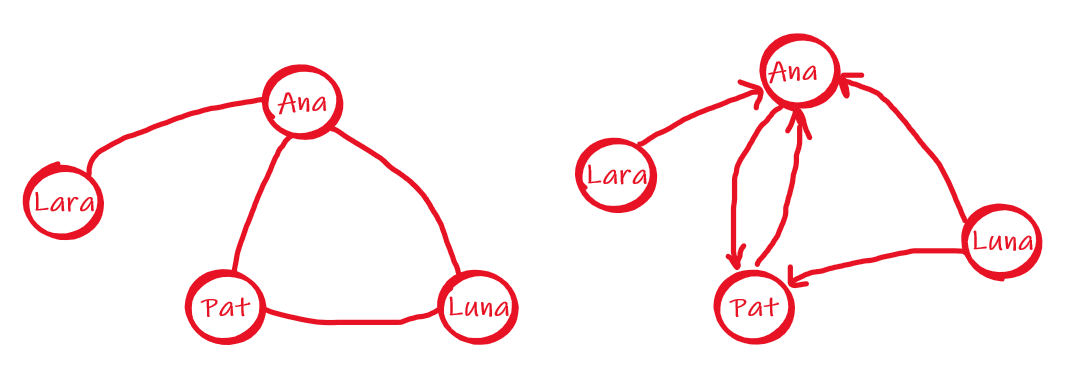
\includegraphics[scale=0.5]{Figuras/facetwitter.png}\\

\end{ftst}


%=====

\begin{ftst}{Multigrafo}{Teoria dos grafos}
\justifying
Um \textbf{multigrafo} é um grafo que possui mais de uma aresta interligando os mesmos dois vértices (arestas múltiplas ou arestas paralelas). 
\vone
Formalmente, um multigrafo $G = (V,E,f$ é composto por um conjunto de vértices $V$, um conjunto de arestas $E$ e uma função $f$:
\vone
\centering
\huge
$f: \{E \rightarrow v_i, v_j \in V$ e $v_i \neq v_j \}$




\tikzset{every picture/.style={line width=0.75pt}} %set default line width to 0.75pt        

\begin{tikzpicture}[x=0.75pt,y=0.75pt,yscale=-1,xscale=1]
%uncomment if require: \path (0,129); %set diagram left start at 0, and has height of 129

%Shape: Ellipse [id:dp6612682211216279] 
\draw  [draw opacity=0][fill={rgb, 255:red, 21; green, 117; blue, 231 }  ,fill opacity=1 ] (91.33,19.19) .. controls (91.33,11.9) and (97.66,6) .. (105.48,6) .. controls (113.29,6) and (119.63,11.9) .. (119.63,19.19) .. controls (119.63,26.47) and (113.29,32.37) .. (105.48,32.37) .. controls (97.66,32.37) and (91.33,26.47) .. (91.33,19.19) -- cycle ;
%Shape: Ellipse [id:dp6477719688590755] 
\draw  [draw opacity=0][fill={rgb, 255:red, 21; green, 117; blue, 231 }  ,fill opacity=1 ] (138.79,63.42) .. controls (138.79,56.13) and (145.13,50.23) .. (152.95,50.23) .. controls (160.76,50.23) and (167.1,56.13) .. (167.1,63.42) .. controls (167.1,70.7) and (160.76,76.6) .. (152.95,76.6) .. controls (145.13,76.6) and (138.79,70.7) .. (138.79,63.42) -- cycle ;
%Shape: Ellipse [id:dp9192783983743278] 
\draw  [draw opacity=0][fill={rgb, 255:red, 21; green, 117; blue, 231 }  ,fill opacity=1 ] (91.33,105.39) .. controls (91.33,98.11) and (97.66,92.21) .. (105.48,92.21) .. controls (113.29,92.21) and (119.63,98.11) .. (119.63,105.39) .. controls (119.63,112.68) and (113.29,118.58) .. (105.48,118.58) .. controls (97.66,118.58) and (91.33,112.68) .. (91.33,105.39) -- cycle ;
%Shape: Ellipse [id:dp7681323151778388] 
\draw  [draw opacity=0][fill={rgb, 255:red, 21; green, 117; blue, 231 }  ,fill opacity=1 ] (46.27,63.42) .. controls (46.27,56.13) and (52.61,50.23) .. (60.42,50.23) .. controls (68.24,50.23) and (74.58,56.13) .. (74.58,63.42) .. controls (74.58,70.7) and (68.24,76.6) .. (60.42,76.6) .. controls (52.61,76.6) and (46.27,70.7) .. (46.27,63.42) -- cycle ;
%Straight Lines [id:da25711558784107824] 
\draw    (69.02,52.63) -- (94.77,27.9) ;
%Straight Lines [id:da9045557667165924] 
\draw    (69.02,72.87) -- (94.77,97.61) ;
%Straight Lines [id:da2028668571778729] 
\draw    (115.69,96.86) -- (144.65,72.87) ;
%Straight Lines [id:da4492549999941824] 
\draw    (147.07,50.39) -- (117.3,25.65) ;
%Straight Lines [id:da21515438842402612] 
\draw    (74.58,63.42) -- (138.79,63.42) ;
%Straight Lines [id:da7967010965789647] 
\draw    (105.48,92.21) -- (105.48,32.37) ;
%Curve Lines [id:da9416584479372687] 
\draw    (48.83,56.23) .. controls (39.26,24.9) and (61.2,7.37) .. (93.97,11.41) ;
%Curve Lines [id:da00818700789856841] 
\draw    (96.38,115.6) .. controls (57.76,133.6) and (32.01,94.61) .. (49.71,72.13) ;




\end{tikzpicture}\\


\end{ftst}

%=====

\begin{ftst}{Pseudogarfo}{Teoria dos grafos}
\justifying
Um pseudografo é um multigrafo com a condição $v_i \neq v_j$ removida na função $f$, ou seja, um vértice pode ser unido a ele mesmo por uma aresta (laço).
\vone
\vone
\centering


\tikzset{every picture/.style={line width=0.75pt}} %set default line width to 0.75pt        

\begin{tikzpicture}[x=0.75pt,y=0.75pt,yscale=-1,xscale=1]
%uncomment if require: \path (0,126); %set diagram left start at 0, and has height of 126

%Shape: Ellipse [id:dp10750631087430529] 
\draw  [draw opacity=0][fill={rgb, 255:red, 21; green, 117; blue, 231 }  ,fill opacity=1 ] (60.33,20.19) .. controls (60.33,12.9) and (66.66,7) .. (74.48,7) .. controls (82.29,7) and (88.63,12.9) .. (88.63,20.19) .. controls (88.63,27.47) and (82.29,33.37) .. (74.48,33.37) .. controls (66.66,33.37) and (60.33,27.47) .. (60.33,20.19) -- cycle ;
%Shape: Ellipse [id:dp18448730365885613] 
\draw  [draw opacity=0][fill={rgb, 255:red, 21; green, 117; blue, 231 }  ,fill opacity=1 ] (107.79,64.42) .. controls (107.79,57.13) and (114.13,51.23) .. (121.95,51.23) .. controls (129.76,51.23) and (136.1,57.13) .. (136.1,64.42) .. controls (136.1,71.7) and (129.76,77.6) .. (121.95,77.6) .. controls (114.13,77.6) and (107.79,71.7) .. (107.79,64.42) -- cycle ;
%Shape: Ellipse [id:dp12970138599304226] 
\draw  [draw opacity=0][fill={rgb, 255:red, 21; green, 117; blue, 231 }  ,fill opacity=1 ] (60.33,106.39) .. controls (60.33,99.11) and (66.66,93.21) .. (74.48,93.21) .. controls (82.29,93.21) and (88.63,99.11) .. (88.63,106.39) .. controls (88.63,113.68) and (82.29,119.58) .. (74.48,119.58) .. controls (66.66,119.58) and (60.33,113.68) .. (60.33,106.39) -- cycle ;
%Shape: Ellipse [id:dp28352645347266736] 
\draw  [draw opacity=0][fill={rgb, 255:red, 21; green, 117; blue, 231 }  ,fill opacity=1 ] (15.27,64.42) .. controls (15.27,57.13) and (21.61,51.23) .. (29.42,51.23) .. controls (37.24,51.23) and (43.58,57.13) .. (43.58,64.42) .. controls (43.58,71.7) and (37.24,77.6) .. (29.42,77.6) .. controls (21.61,77.6) and (15.27,71.7) .. (15.27,64.42) -- cycle ;
%Straight Lines [id:da39697278104923206] 
\draw    (38.02,53.63) -- (63.77,28.9) ;
%Straight Lines [id:da6218967074559845] 
\draw    (38.02,73.87) -- (63.77,98.61) ;
%Straight Lines [id:da7056326038158895] 
\draw    (84.69,97.86) -- (113.65,73.87) ;
%Straight Lines [id:da09345796540583517] 
\draw    (116.07,51.39) -- (86.3,26.65) ;
%Straight Lines [id:da07714315548852912] 
\draw    (43.58,64.42) -- (107.79,64.42) ;
%Straight Lines [id:da25098017047871024] 
\draw    (74.48,93.21) -- (74.48,33.37) ;
%Curve Lines [id:da5784233547387851] 
\draw    (17.83,57.23) .. controls (8.26,25.9) and (30.2,8.37) .. (62.97,12.41) ;
%Curve Lines [id:da9415713722574512] 
\draw    (65.38,116.6) .. controls (26.76,134.6) and (1.01,95.61) .. (18.71,73.13) ;
%Curve Lines [id:da15023932434498688] 
\draw    (128.11,54.08) .. controls (182.26,21.93) and (193.26,99.55) .. (127.11,75.08) ;




\end{tikzpicture}\\


\end{ftst}

%=====

\begin{ftst}{Incidência}{Teoria dos grafos}
\justifying
\begin{itemize}
    \item Seja dois vértices $v_i$ e $v_j$, e uma aresta $a_k = (v_i,v_j)$.
    \item A aresta $a_k$ é dita \textcolor{red}{\textbf{incidente}} a ambos vértices $v_i$ e $v_j$.
    \item Duas arestas não paralelas que são incidentes a um mesmo vértice são ditas \textcolor{yellow}{\textbf{adjacentes}}.
    \item Dois vértices que são ligados por uma mesma arestas também são ditos \textcolor{green}{\textbf{adjacentes}}. 
\end{itemize}
\vone
\vone
\centering




\tikzset{every picture/.style={line width=0.75pt}} %set default line width to 0.75pt        

\begin{tikzpicture}[x=0.75pt,y=0.75pt,yscale=-1,xscale=1]
%uncomment if require: \path (0,143); %set diagram left start at 0, and has height of 143

%Shape: Circle [id:dp04362587289462838] 
\draw  [draw opacity=0][fill={rgb, 255:red, 21; green, 117; blue, 231 }  ,fill opacity=1 ] (41.82,107.59) .. controls (41.82,97.88) and (49.69,90) .. (59.41,90) .. controls (69.12,90) and (77,97.88) .. (77,107.59) .. controls (77,117.31) and (69.12,125.18) .. (59.41,125.18) .. controls (49.69,125.18) and (41.82,117.31) .. (41.82,107.59) -- cycle ;
%Shape: Circle [id:dp9127487846171529] 
\draw  [draw opacity=0][fill={rgb, 255:red, 21; green, 117; blue, 231 }  ,fill opacity=1 ] (95.82,30.59) .. controls (95.82,20.88) and (103.69,13) .. (113.41,13) .. controls (123.12,13) and (131,20.88) .. (131,30.59) .. controls (131,40.31) and (123.12,48.18) .. (113.41,48.18) .. controls (103.69,48.18) and (95.82,40.31) .. (95.82,30.59) -- cycle ;
%Shape: Circle [id:dp1516086263423222] 
\draw  [draw opacity=0][fill={rgb, 255:red, 21; green, 117; blue, 231 }  ,fill opacity=1 ] (175.82,82.59) .. controls (175.82,72.88) and (183.69,65) .. (193.41,65) .. controls (203.12,65) and (211,72.88) .. (211,82.59) .. controls (211,92.31) and (203.12,100.18) .. (193.41,100.18) .. controls (183.69,100.18) and (175.82,92.31) .. (175.82,82.59) -- cycle ;
%Curve Lines [id:da39429388955581657] 
\draw [color={rgb, 255:red, 93; green, 164; blue, 16 }  ,draw opacity=1 ][line width=1.5]  [dash pattern={on 1.69pt off 2.76pt}]  (38.26,82.08) .. controls (29.08,59.66) and (23.62,20.51) .. (81.32,21.91) ;
\draw [shift={(84,22)}, rotate = 182.55] [color={rgb, 255:red, 93; green, 164; blue, 16 }  ,draw opacity=1 ][line width=1.5]    (14.21,-4.28) .. controls (9.04,-1.82) and (4.3,-0.39) .. (0,0) .. controls (4.3,0.39) and (9.04,1.82) .. (14.21,4.28)   ;
\draw [shift={(39.6,85.18)}, rotate = 245.56] [color={rgb, 255:red, 93; green, 164; blue, 16 }  ,draw opacity=1 ][line width=1.5]    (14.21,-4.28) .. controls (9.04,-1.82) and (4.3,-0.39) .. (0,0) .. controls (4.3,0.39) and (9.04,1.82) .. (14.21,4.28)   ;
%Straight Lines [id:da4074643230835915] 
\draw    (69.6,92.18) -- (103.6,46.18) ;
%Straight Lines [id:da8791514893393153] 
\draw    (180.6,69.18) -- (131.6,38.18) ;
%Curve Lines [id:da6036233288375135] 
\draw [color={rgb, 255:red, 237; green, 12; blue, 39 }  ,draw opacity=1 ][line width=1.5]  [dash pattern={on 1.69pt off 2.76pt}]  (80.82,95.92) .. controls (113.53,93.22) and (110.88,92.04) .. (114.32,56.02) ;
\draw [shift={(114.6,53.18)}, rotate = 455.71] [color={rgb, 255:red, 237; green, 12; blue, 39 }  ,draw opacity=1 ][line width=1.5]    (14.21,-4.28) .. controls (9.04,-1.82) and (4.3,-0.39) .. (0,0) .. controls (4.3,0.39) and (9.04,1.82) .. (14.21,4.28)   ;
\draw [shift={(77.6,96.18)}, rotate = 355.36] [color={rgb, 255:red, 237; green, 12; blue, 39 }  ,draw opacity=1 ][line width=1.5]    (14.21,-4.28) .. controls (9.04,-1.82) and (4.3,-0.39) .. (0,0) .. controls (4.3,0.39) and (9.04,1.82) .. (14.21,4.28)   ;
%Curve Lines [id:da3678012255650336] 
\draw [color={rgb, 255:red, 247; green, 228; blue, 5 }  ,draw opacity=1 ][line width=1.5]  [dash pattern={on 1.69pt off 2.76pt}]  (118.68,90.37) .. controls (142.33,99.51) and (157.97,105.29) .. (162.29,69.98) ;
\draw [shift={(162.6,67.18)}, rotate = 455.71] [color={rgb, 255:red, 247; green, 228; blue, 5 }  ,draw opacity=1 ][line width=1.5]    (14.21,-4.28) .. controls (9.04,-1.82) and (4.3,-0.39) .. (0,0) .. controls (4.3,0.39) and (9.04,1.82) .. (14.21,4.28)   ;
\draw [shift={(115.6,89.18)}, rotate = 21.04] [color={rgb, 255:red, 247; green, 228; blue, 5 }  ,draw opacity=1 ][line width=1.5]    (14.21,-4.28) .. controls (9.04,-1.82) and (4.3,-0.39) .. (0,0) .. controls (4.3,0.39) and (9.04,1.82) .. (14.21,4.28)   ;

% Text Node
\draw (132,8.4) node [anchor=north west][inner sep=0.75pt]    {$v_{1}$};
% Text Node
\draw (27,119.4) node [anchor=north west][inner sep=0.75pt]    {$v_{2}$};
% Text Node
\draw (215,87.99) node [anchor=north west][inner sep=0.75pt]    {$v_{3}$};
% Text Node
\draw (90,67.4) node [anchor=north west][inner sep=0.75pt]    {$a_{1}$};
% Text Node
\draw (156,38.4) node [anchor=north west][inner sep=0.75pt]    {$a_{2}$};


\end{tikzpicture}\\


\end{ftst}

%=====

\begin{ftst}{Grau de um Vértice}{Teoria dos grafos}
\justifying
O grau de um vértice é definido como o número de arestas incidentes em tal vértice.
\vone
\vone
\centering


\tikzset{every picture/.style={line width=0.75pt}} %set default line width to 0.75pt        

\begin{tikzpicture}[x=0.75pt,y=0.75pt,yscale=-1,xscale=1]
%uncomment if require: \path (0,177); %set diagram left start at 0, and has height of 177

%Shape: Ellipse [id:dp8878451264053866] 
\draw  [draw opacity=0][fill={rgb, 255:red, 21; green, 117; blue, 231 }  ,fill opacity=1 ] (68.33,18.19) .. controls (68.33,10.9) and (74.66,5) .. (82.48,5) .. controls (90.29,5) and (96.63,10.9) .. (96.63,18.19) .. controls (96.63,25.47) and (90.29,31.37) .. (82.48,31.37) .. controls (74.66,31.37) and (68.33,25.47) .. (68.33,18.19) -- cycle ;
%Shape: Ellipse [id:dp2916294149093952] 
\draw  [draw opacity=0][fill={rgb, 255:red, 21; green, 117; blue, 231 }  ,fill opacity=1 ] (137.27,83.42) .. controls (137.27,76.13) and (143.61,70.23) .. (151.42,70.23) .. controls (159.24,70.23) and (165.58,76.13) .. (165.58,83.42) .. controls (165.58,90.7) and (159.24,96.6) .. (151.42,96.6) .. controls (143.61,96.6) and (137.27,90.7) .. (137.27,83.42) -- cycle ;
%Shape: Ellipse [id:dp3230435826467881] 
\draw  [draw opacity=0][fill={rgb, 255:red, 21; green, 117; blue, 231 }  ,fill opacity=1 ] (70.33,149.19) .. controls (70.33,141.9) and (76.66,136) .. (84.48,136) .. controls (92.29,136) and (98.63,141.9) .. (98.63,149.19) .. controls (98.63,156.47) and (92.29,162.37) .. (84.48,162.37) .. controls (76.66,162.37) and (70.33,156.47) .. (70.33,149.19) -- cycle ;
%Shape: Ellipse [id:dp43124705110127093] 
\draw  [draw opacity=0][fill={rgb, 255:red, 21; green, 117; blue, 231 }  ,fill opacity=1 ] (4.27,83.42) .. controls (4.27,76.13) and (10.61,70.23) .. (18.42,70.23) .. controls (26.24,70.23) and (32.58,76.13) .. (32.58,83.42) .. controls (32.58,90.7) and (26.24,96.6) .. (18.42,96.6) .. controls (10.61,96.6) and (4.27,90.7) .. (4.27,83.42) -- cycle ;
%Curve Lines [id:da2175749921862662] 
\draw    (18.42,70.23) .. controls (31.15,39.25) and (32.15,26.25) .. (68.33,18.19) ;
%Curve Lines [id:da3475393637016071] 
\draw    (70.33,149.19) .. controls (48.33,153.19) and (15.42,129.6) .. (18.42,96.6) ;
%Curve Lines [id:da8464775768749004] 
\draw    (77.15,138.25) .. controls (73.83,111.49) and (70.73,97.08) .. (30.15,88.25) ;
%Curve Lines [id:da2560797041651943] 
\draw    (27.15,75.25) .. controls (59.15,69.25) and (78.15,42.25) .. (77.15,30.25) ;
%Curve Lines [id:da7980507121214329] 
\draw    (151.42,70.23) .. controls (154.15,49.25) and (126.63,15.19) .. (96.63,18.19) ;
%Curve Lines [id:da8344460663280768] 
\draw    (151.42,96.6) .. controls (152.15,140.25) and (125.63,150.19) .. (98.63,149.19) ;
%Straight Lines [id:da00593623081886796] 
\draw    (32.58,83.42) -- (137.27,83.42) ;

% Text Node
\draw (8,51) node [anchor=north west][inner sep=0.75pt]  [font=\large] [align=left] {\textbf{\textcolor[rgb]{0.95,0.05,0.05}{5}}};
% Text Node
\draw (100.63,23.19) node [anchor=north west][inner sep=0.75pt]  [font=\large] [align=left] {\textbf{\textcolor[rgb]{0.95,0.05,0.05}{3}}};
% Text Node
\draw (170.63,73.19) node [anchor=north west][inner sep=0.75pt]  [font=\large] [align=left] {\textbf{\textcolor[rgb]{0.95,0.05,0.05}{3}}};
% Text Node
\draw (97.63,125.19) node [anchor=north west][inner sep=0.75pt]  [font=\large] [align=left] {\textbf{\textcolor[rgb]{0.95,0.05,0.05}{3}}};


\end{tikzpicture}\\


\end{ftst}

%=====

\begin{ftst}{Exercício}{Teoria dos grafos}
\justifying
\textbf{Teorema 1}: a soma dos graus de todos os vértices de um grafo G é igual a duas vezes o número de arestas do grafo.
\vone
\textbf{Teorema 2}: o número de vértices de grau ímpar de um grafo é sempre par.
\vone
\textbf{Pergunta}: Se G é um grafo com 14 vértices e 25 arestas, cujos vértices têm grau 3 ou 5, quantos vértices tem grau 3 e quantos tem grau 5?



\end{ftst}

%=====



\end{document}